\begin{figure}[htbp]
\centering
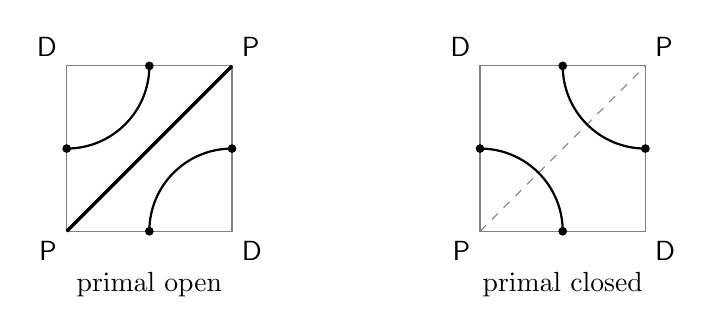
\begin{tikzpicture}[scale=1.05]
 \begin{scope}
  \draw[gray] (0,0) rectangle (2,2);
  \draw[very thick] (0,0)--(2,2);
  \draw[thick] (0,1) arc[start angle=-90,end angle=0,radius=1];
  \draw[thick] (1,0) arc[start angle=180,end angle=90,radius=1];
  \node[below left] at (0,0) {$\mathsf P$};
  \node[above right] at (2,2) {$\mathsf P$};
  \node[above left] at (0,2) {$\mathsf D$};
  \node[below right] at (2,0) {$\mathsf D$};
  \foreach \x/\y in {0/1,1/0,2/1,1/2}
    \fill (\x,\y) circle (1.5pt);
  \node at (1,-.65) {primal open};
 \end{scope}
 \begin{scope}[xshift=5cm]
  \draw[gray] (0,0) rectangle (2,2);
  \draw[dashed,gray] (0,0)--(2,2);
  \draw[thick] (1,0) arc[start angle=0,end angle=90,radius=1];
  \draw[thick] (2,1) arc[start angle=-90,end angle=-180,radius=1];
  \node[below left] at (0,0) {$\mathsf P$};
  \node[above right] at (2,2) {$\mathsf P$};
  \node[above left] at (0,2) {$\mathsf D$};
  \node[below right] at (2,0) {$\mathsf D$};
  \foreach \x/\y in {0/1,1/0,2/1,1/2}
    \fill (\x,\y) circle (1.5pt);
  \node at (1,-.65) {primal closed};
 \end{scope}
\end{tikzpicture}
\caption{The two tile switches. The solid diagonal is an open primal
edge; the dashed diagonal records the absent primal edge. The curved
arcs specify the pairing of ports and hence the order of strand
occurrences when a medial vertex is visited twice.}
\label{prelim:switch-figure}
\end{figure}
